\documentclass[12pt]{article}
\usepackage[utf8]{inputenc}
\usepackage[margin=1in,bottom=1.5in,a4paper]{geometry}
\usepackage{tikz}
\usepackage{amsmath}
\usepackage{amssymb}
\usepackage{multicol}
\usepackage{xcolor}
\usepackage{tabularx}
\usepackage{mathtools}
\usepackage{ textcomp }
\usepackage{graphicx}
\usepackage{ stmaryrd }
\usepackage{hyperref}
\usepackage{ marvosym }
\usepackage{ dsfont }
\usepackage{ulem}
\tolerance=1000
\usepackage{fancyhdr}
\pagestyle{fancy}
\headheight 50pt

\renewcommand{\thesection}{\Alph{section}}

%edit header and footer
\fancypagestyle{firstpage}{
  \lhead{X-as-a-Service cloud assets}
  \chead{\textbf{\Large Azure}}
  \rhead{CySec Project '21}
}
\lhead{}
\rhead{X-as-a-Service cloud assets}

\cfoot{}
\rfoot{\small\thepage}

\begin{document}
\thispagestyle{firstpage}

\section*{Azure for Students}
Overview on Azure and their services (kinda ranked after use-cases)
\begin{enumerate}
    \item Compute: VMs (IaaS), Container Instances (virtualised Applicationenvironments), App Service, Functions
    \item Networking (VPN,...)
    \item Storage
    \item Mobile services (apps,...)
    \item Databases
    \item Web (Web apps, ...)
    \item IoT (manage all IoT assets, ...)
    \item BigData (cluster services, ...)
    \item AI services and Machine Learning
    \item DevOps
\end{enumerate}


\subsection*{Notes}
\begin{itemize}
    \item CA from my static website: Microsoft Azure TLS Issuing CA 01
    \item Easy to differentiate between VM and Containers: VM virtualise the hardware, containers the OS
    \item \verb|azurewebsites.net|, \verb|azurestaticapps.net| as domain ending
    \item Static and web apps can be set up with the help of Git \\ 
    $\rightarrow$ learning something via Git Accounts?
    \item Possibilities to secure Azure: SecurityCenter, Sentinel, 
\end{itemize}

\subsection*{To be checked out:}
\url{https://sonraisecurity.com/blog/attackers-find-aws-s3-bucket-with-17m-users/} \\ \\




\newpage
\subsection*{Most common mistakes with Azure}
\begin{itemize}

    \item \textbf{Misconfiguration of Roles \& Administration:} \footnote{\url{https://blog.e-zest.com/here-are-10-most-common-mistakes-while-managing-azure-cloud}} \footnote{\url{https://www.lightstream.tech/top-5-azure-mistakes-your-security-team-is-making/}} \footnote{\url{https://www.viacode.com/most-common-azure-security-problems/}}
    
    making everyone as (co-)administrator in the Azure subscription. Team members often times remove or delete the Azure components, which creates lot of impact on overall application and ruins the stability of the environment. Members also unknowingly keep on provisioning Azure resources for research and evaluation purpose which causes a huge expenditure. Data Storage Access Misconfig: a user can set permissions that expose data to the entire internet in "Azure Storage" \textbf{(try to do that!)} 

    $\rightarrow$ provide users only with the amount of permission they need to do their job! \\
    RBAC (Role Based Access Control) or ARM (Azure Resource Manager) or MFA (Multi-Factor auth.) 


    \item \textbf{Choosing incorrect specifications (of Azure VM) \& not securing access points} \footnotemark[1] \footnote{\url{https://techgyo.com/5-common-microsoft-azure-security-mistake}} \\
    All aspects like overall user load, nature of the application and geography of the users must be considered by enterprises and individuals hosting their applications, before designing the infrastructure.
    Not securing access points to the clouds, allowing users to access the VM from any machine, anywhere.
    
    
    \item \textbf{Billing of over usage} \footnotemark[1] \\
    They keep running their Azure instances, even if they are not in use or when purpose is served. \\
    $\rightarrow$ keep resources in off-state or delete them once you no longer need them.
    
    
    \item \textbf{Weak, mismanaged Passwords:} \footnotemark[2] \footnotemark[4] \\ 
    Improper password management and bad password habits. Microsoft reports 10 million username/password pair attacks per day.
    
    
    \item \textbf{Misconfig/not enabling of Security/Managing Controls:} \footnotemark[2] \\ 
    Failed to turn on the logging feature. Necessary to permit access visibility but also to see who is accessing and managing the subscription.
    Failing to enable Azures security center and its native security tools (\textbf{check this out!}) \\
    \textbf{TODO}: subnets should not be assigned to a public IP that could open unwanted ports. (Network Security Groups (NSGs)) NSGs control access by permitting or denying network traffic via communication between different workloads on a vNET, network connectivity from on-site environment into Azure, or direct internet connection.
    
    \item \textbf{Lack of Oversight / Security Monitoring:} \footnotemark[2] \footnotemark[3] \\ 
    Missing ongoing management and security (often times just in the beginning and then not covered anymore)
    Security vulnerabilities result when Azure users don’t understand what they are responsible for and the tools and services Azure provides to help them. 
    \begin{center}
        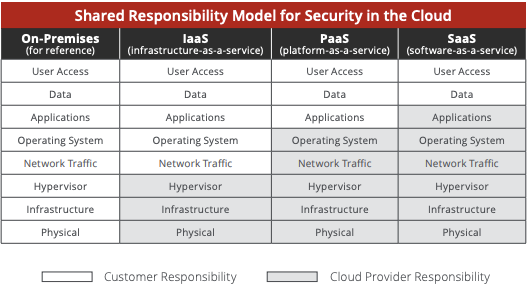
\includegraphics[scale=0.5]{McAfee_Responsibility_Model.png} \footnotemark[5] 
    \end{center}
    
    
    \item \textbf{Cloud misconfiguration:} \footnotemark[3] \\
    Especially the misconfiguration of databases and object storage services. (linked there - \url{https://www.mcafee.com/enterprise/en-us/assets/skyhigh/white-papers/cloud-adoption-risk-report-2019.pdf})
    
    \item \textbf{Not encrypting data at rest:} \footnotemark[3] \\ 
    blobs are encrypted by default, but VM disks are not, creating vuln. User have to enable disk encryption on their own (for free!).
    
    \item \textbf{Not managing patches correctly:} \footnotemark[4] \\
    Not applying a patch at all or do it only half the way.
    
    \item \textbf{Not testing security or taking it for granted:} \footnotemark[4] \footnotemark[1] \\ 
    Users should use penetration testers (microsoft has a policy governing such tests).
    Even though Microsoft secures the platform, it can't protect against e.g. weak passwords
    
    \item \textbf{Not opting for Microsoft support option} \footnotemark[1] \\
    To save costs, companies try to avoid the support when purchasing the Azure subscription. 
    But it can happen, that even a high skilled employer isn't able to e.g. shut down a VM. The support however can do this. If enterprises have not chosen the appropriate support option then there might be a huge impact. 
    
    \item \textbf{McAfee Report} \footnote{\url{https://www.mcafee.com/enterprise/en-us/assets/skyhigh/white-papers/cloud-adoption-risk-report-2019.pdf}} \\
    More and more files contain sensitive information and too many are publicly accessible. Enterprise organizations have an average of 14 misconfigured IaaS/PaaS instances.
    
\end{itemize}


\newpage
\section*{Azure Key Vault}
%\verb|"<your-unique-storage-account-name>" = storageforkeyvault|

%\verb|"<your-unique-keyvault-name>" = super-secure-keyvault|

Search for \verb|.vault.azure.net| websites (e.g. Dorking: \verb|site:*.vault.azure.net/|)\\
$\rightarrow$ no results, aren't listed...

Resolve the key vault uri (\url{https://super-secure-keyvault.vault.azure.net/}, \url{https://aiskeyrun.vault.azure.net}) \\
$\rightarrow$ runs on \verb|51.116.154.67| and \verb|ASN 8075|


%\newpage
\section*{Azures SecurityCenter}


\end{document}
